\documentclass[11pt]{article}

\usepackage[a4paper,margin=24mm]{geometry}
\usepackage[T1]{fontenc}
\usepackage[utf8]{inputenc}
\usepackage{lmodern}
\usepackage{microtype}
\usepackage{amsmath,amssymb}
\usepackage{booktabs}
\usepackage{graphicx}
\usepackage{array}
\usepackage{enumitem}
\usepackage{xcolor}
\usepackage[hidelinks]{hyperref}

\definecolor{navy}{HTML}{183153}
\definecolor{lightblue}{HTML}{EAF2F8}
\definecolor{orange}{HTML}{C44900}
\setlength{\parindent}{0pt}
\setlength{\parskip}{0.55em}
\setlist{nosep,leftmargin=*}
\renewcommand{\arraystretch}{1.13}

\title{\textbf{Five-Seed Reproducibility Study of a Library-Based\\CartPole DAgger Baseline}}
\author{Experimental supplement to \emph{Experimental Analysis of DAgger}\\
Nowshin Tabassum, Intesur Ahmed, and Md. Rakibul Hassan}
\date{21 August 2026}

\begin{document}
\maketitle

\begin{abstract}
This report answers whether repeated runs of the current CartPole DAgger baseline can produce different results. Five independent training seeds (0--4) were run. Each seed trained a new proximal policy optimization (PPO) expert, initialized a new behavior-cloning learner, collected new DAgger trajectories, and performed new optimization. Every checkpoint was evaluated without expert assistance on the same 20 deterministic evaluation episodes. After the first expert-controlled data round, the learner's mean return differed substantially by seed: the five-seed mean was 191.29, the sample standard deviation was 97.19, and the 95\% Student-$t$ confidence interval was [70.61, 311.97]. After round 1, all five seeds reached the CartPole-v1 return ceiling of 500 and remained there through round 5. Thus, multiple runs \emph{did} change early learning, while the final outcome was identical under this evaluation protocol. The final ceiling result is evidence of consistency in this baseline, but it is not proof that all seeds, initial states, experts, or DAgger variants will always score 500.
\end{abstract}

\section{Scope and relationship to the project plan}

The supplied project document proposes DAgger experiments on Stanford OCR and CartPole, with a rule-based CartPole expert
\[
\pi^*(s)=\mathbb{1}\!\left[\theta+0.6\dot{\theta}+0.02\dot{x}>0\right].
\]
The experiment reported here is the intentionally separate \texttt{imitation\_library\_cartpole} reference baseline. It uses a newly trained PPO expert for each seed and the \texttt{imitation} package's \texttt{SimpleDAggerTrainer}. It does \textbf{not} consume the fixed rule-expert CSV and does not yet evaluate OCR, behavior cloning versus DAgger under a matched label budget, retention ablations, uncertainty querying, or partial observability. Consequently, these measurements validate the library-based training and evaluation pipeline; they are not the final results of the complete project or its proposed novelty.

\section{Research question}

The question is: \emph{If the complete training procedure is repeated, do different random seeds produce different CartPole returns?} A proper repetition must retrain the models and recollect the data. Merely evaluating one saved policy five times would measure variation in evaluation episodes, not variation in learning. Here, one training seed is the experimental unit.

The five seeds affect PPO parameter initialization and minibatches, the PPO training environment, the DAgger collection environment, the expert/learner mixing decisions, the initial behavior-cloning network, and behavior-cloning minibatches. Evaluation randomness was held fixed so that learner checkpoints faced a common test.

\section{Methodology}

\subsection{Environment and return}

The environment was Gymnasium \texttt{CartPole-v1}. Its observation is $s=(x,\dot{x},\theta,\dot{\theta})\in\mathbb{R}^4$, and its two actions push the cart left or right. The agent receives $+1$ for each surviving step. An episode terminates after failure or is truncated at the 500-step horizon, so the maximum undiscounted return is 500.

\subsection{Independent PPO experts}

For every training seed $k\in\{0,1,2,3,4\}$, a new Stable-Baselines3 PPO expert was trained on a CartPole environment seeded by $k$. The requested budget was 50,000 environment steps. PPO collects complete 2,048-step rollouts, so each run actually completed 51,200 steps. The policy and value networks used two 64-unit tanh layers. Other relevant defaults were: learning rate $3\times10^{-4}$, batch size 64, 10 optimization epochs per update, discount $\gamma=0.99$, GAE parameter $\lambda=0.95$, and clipping parameter 0.2. Each expert was evaluated deterministically for 20 episodes using common evaluation seed 10,000.

The PPO expert is a practical library baseline, not the analytic rule-based controller specified by the main project PDF. Keeping this distinction visible prevents two different expert sources from being reported as one experiment.

\subsection{DAgger learner and data aggregation}

The learner was the \texttt{imitation} package's default \texttt{FeedForward32Policy}: two shared 32-unit tanh hidden layers and a two-action output. Behavior cloning used Adam with learning rate $10^{-3}$ and batch size 32. After each collection round, the learner was trained for four epochs on the complete aggregated demonstration set.

At round $i$, data were collected with the mixture
\[
\pi_i=\beta_i\pi^*+(1-\beta_i)\hat\pi_i,
\qquad \beta_i=0.5^i.
\]
Here, $\beta_i$ is the probability that the expert physically controls a collection step. It is a probability, not a claim that the realized fraction of expert-controlled steps is exactly $\beta_i$. Dense-supervision DAgger still queries the expert for a label at \emph{every} visited state, including states reached while the learner controls the environment.

Each collection round required at least three complete episodes and at least 500 steps. All collected episodes in these runs reached the 500-step horizon; therefore, each round added $3\times500=1{,}500$ labeled transitions. The requested DAgger budget was 8,000 steps, but the trainer may stop only after a complete round. Six rounds produced 9,000 transitions in total. This is expected overshoot, not a counting error.

Round 0 used $\beta_0=1$: its collection trajectories were physically driven entirely by the expert. The checkpoint evaluated after training on those first 1,500 labels is therefore a behavior-cloning-like initial checkpoint. Round 1 used $\beta_1=0.5$, exposing data collection to learner-induced states before retraining.

\subsection{Evaluation protocol}

After every round, the learner acted \textbf{alone}: no expert actions were mixed into evaluation. Actions were deterministic. A fresh environment was reconstructed with seed 40,000 for every checkpoint, producing the same 20-episode initial-condition sequence for every round and every training seed. This correction matters because changing the evaluation seed at each round confounds policy improvement with easier or harder initial states.

A separate final evaluation used 20 episodes from common seed 30,000. Thus, the round curve and final test use different fixed episode sequences. Evaluation seeds were never used for PPO or DAgger training.

\begin{table}[ht]
\centering
\caption{Fixed experimental configuration.}
\small
\begin{tabular}{@{}p{0.40\linewidth}p{0.51\linewidth}@{}}
\toprule
Item & Setting \\
\midrule
Training seeds & 0, 1, 2, 3, 4 \\
Environment & CartPole-v1; maximum return 500 \\
Expert & Independent PPO model per training seed \\
PPO budget & 50,000 requested; 51,200 actual steps \\
DAgger schedule & $\beta_i=0.5^i$, rounds 0--5 \\
Collection per round & 3 complete episodes; 1,500 transitions \\
DAgger budget & 8,000 requested; 9,000 actual labeled transitions \\
Learner update & Aggregate all past data; 4 BC epochs per round \\
Round evaluation & 20 episodes, common seed 40,000 \\
Final evaluation & 20 episodes, common seed 30,000 \\
Expert evaluation & 20 episodes, common seed 10,000 \\
\bottomrule
\end{tabular}
\end{table}

\subsection{Statistical summary}

Let $\bar R_{ik}$ be the mean return across 20 fixed evaluation episodes at round $i$ for training seed $k$. The reported round mean is the average of the five independent training-seed means. Across-seed uncertainty uses
\[
\bar R_i \ \pm\ t_{0.975,4}\frac{s_i}{\sqrt{5}},
\qquad t_{0.975,4}=2.7764,
\]
where $s_i$ is the sample standard deviation of the five values $\bar R_{ik}$. This interval estimates uncertainty from changing the complete training run. It should not be confused with the standard deviation of 20 episode returns for one trained policy. The graph clips confidence bands to the physically possible range $[0,500]$; the numerical table reports the same bounded values here because no interval crosses a boundary except the degenerate ceiling rows.

\section{Results}

\subsection{Raw per-seed checkpoint means}

The first checkpoint varied considerably: seed 1 obtained 331.15, whereas seed 2 obtained 108.10. From round 1 onward, every seed obtained 500.00 on all 20 common round-evaluation episodes.

\begin{table}[ht]
\centering
\caption{Mean return over the 20 fixed round-evaluation episodes. Values are measured, not claimed or manually entered.}
\small
\begin{tabular}{@{}crrrrrr@{}}
\toprule
Seed & R0 & R1 & R2 & R3 & R4 & R5 \\
\midrule
0 & 153.45 & 500.00 & 500.00 & 500.00 & 500.00 & 500.00 \\
1 & 331.15 & 500.00 & 500.00 & 500.00 & 500.00 & 500.00 \\
2 & 108.10 & 500.00 & 500.00 & 500.00 & 500.00 & 500.00 \\
3 & 251.50 & 500.00 & 500.00 & 500.00 & 500.00 & 500.00 \\
4 & 112.25 & 500.00 & 500.00 & 500.00 & 500.00 & 500.00 \\
\bottomrule
\end{tabular}
\end{table}

The within-seed episode standard deviations at round 0 were 100.98, 207.06, 37.00, 204.64, and 63.37 for seeds 0--4, respectively. These describe sensitivity to the 20 initial conditions for each particular trained checkpoint. All within-seed episode standard deviations were 0 from round 1 onward because every episode lasted exactly 500 steps.

\subsection{Across-seed aggregate}

\begin{table}[ht]
\centering
\caption{Aggregate performance across five independent training seeds. CI is a two-sided 95\% Student-$t$ interval over seed means.}
\small
\begin{tabular}{@{}crrrrc@{}}
\toprule
Round & $\beta_i$ & Cum. labels & Mean & Seed SD & 95\% CI \\
\midrule
0 & 1.00000 & 1,500 & 191.29 & 97.19 & [70.61, 311.97] \\
1 & 0.50000 & 3,000 & 500.00 & 0.00 & [500.00, 500.00] \\
2 & 0.25000 & 4,500 & 500.00 & 0.00 & [500.00, 500.00] \\
3 & 0.12500 & 6,000 & 500.00 & 0.00 & [500.00, 500.00] \\
4 & 0.06250 & 7,500 & 500.00 & 0.00 & [500.00, 500.00] \\
5 & 0.03125 & 9,000 & 500.00 & 0.00 & [500.00, 500.00] \\
\bottomrule
\end{tabular}
\end{table}

The paired improvement from round 0 to round 1 was 308.71 return points on average. Because every round-1 score was 500, its across-seed sample standard deviation equals the round-0 standard deviation, 97.19; the corresponding 95\% confidence interval for the improvement is [188.03, 429.39]. The evidence therefore supports a large improvement after adding the first mixed-policy collection round in this configuration.

\begin{figure}[ht]
\centering
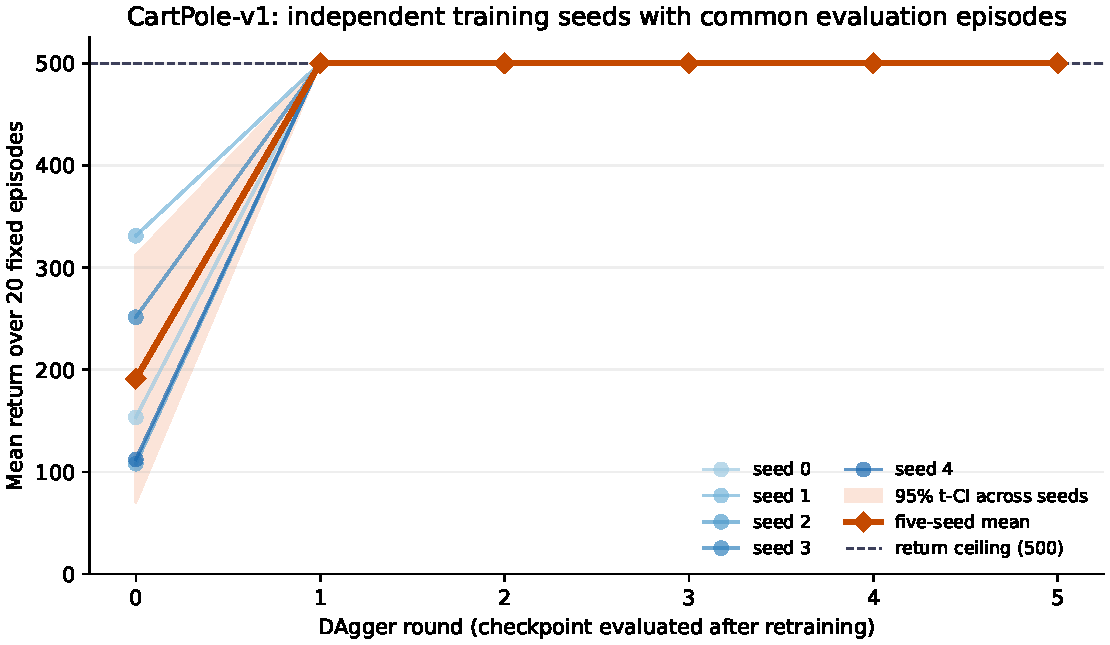
\includegraphics[width=\linewidth]{../analysis/multiseed_learning_curve.pdf}
\caption{Five independently trained learners (blue), their mean (orange), and the 95\% Student-$t$ interval across training-seed means (shaded). The common evaluation episodes isolate training variation. The return ceiling hides any performance difference above the task's maximum.}
\label{fig:curve}
\end{figure}

\subsection{Expert and final-policy checks}

All five independently trained PPO experts scored $500.00\pm0.00$ over their 20 common expert-evaluation episodes. All five final DAgger learners also scored $500.00\pm0.00$ over the separate 20-episode final evaluation sequence. Across the five seed means, both the expert and final learner had mean 500, sample standard deviation 0, and an empirical 95\% interval [500,500]. In total, the final-policy check contains 100 learner episodes, all at the 500-step ceiling.

The zero-width empirical interval does \textbf{not} mean the true uncertainty is mathematically zero. It means that this finite experiment observed no variation at a metric with a hard ceiling. Different evaluation states, more demanding perturbations, fewer demonstrations, a weaker expert, or other training seeds can reveal differences that this test cannot resolve.

\section{Interpretation}

The direct answer is \textbf{yes}: multiple full runs can produce different results. This is visible at round 0, where independent seed means span 108.10--331.15. A single seed-0 curve therefore understated the uncertainty of early learning. The corrected five-seed estimate is 191.29 with a wide interval.

The second observation is that these differences disappear after round 1 under the chosen test. A plausible mechanism is that the first mixed rollout ($\beta=0.5$) adds expert labels on states influenced by learner actions. Training on the combined 3,000 labels then covers enough recovery-relevant CartPole states for every tested learner to solve the 20 common episodes. Later rounds cannot show further improvement because 500 is the maximum return.

This experiment alone cannot separate three explanations for the plateau: (i) DAgger data aggregation reliably solved the task; (ii) CartPole and the PPO expert made the task easy for this learner and data budget; and (iii) the fixed evaluation set was not challenging enough to distinguish later checkpoints. The measurements support consistency within the declared protocol, not universal convergence after one DAgger round.

\section{Limitations and next methodological steps}

\begin{enumerate}
  \item \textbf{Expert mismatch with the project PDF.} This baseline uses PPO. The primary CartPole experiment should repeat the study with the PDF's rule-based expert and compare the two expert sources explicitly.
  \item \textbf{No matched BC control yet.} Round 0 is an initial expert-data checkpoint, but a formal BC baseline should receive a clearly matched dataset or label budget and be evaluated at the same seeds.
  \item \textbf{Ceiling effect.} Return 500 cannot reveal whether one solved policy is more stable than another. Evaluation should add more unseen seeds and controlled disturbances, observation noise, or altered initial-state ranges while preserving a standard CartPole-v1 result.
  \item \textbf{Five seeds are exploratory.} Five runs are much stronger than one, but the round-0 interval remains wide. Ten or more seeds would estimate early learning more precisely if compute permits.
  \item \textbf{Only one environment and metric.} These results do not establish the planned OCR character-accuracy result, the label-budget novelty, data-retention ablation, query-strategy comparisons, or partial-observability study.
  \item \textbf{Dense labels.} The library baseline queries the expert at every visited state. It cannot answer how many labels can be removed; that requires the custom label-budgeted implementation.
\end{enumerate}

The next primary experiment should use the same statistical structure---independent training seeds, common unseen evaluation episodes, learner-only evaluation, raw result retention, and confidence intervals---while replacing the PPO expert with the rule-based controller and adding the matched BC and ablation conditions from the project plan.

\section{Reproducibility and generated artifacts}

The experiment can be resumed safely because existing run directories are never overwritten. From \texttt{Final Project/imitation\_library\_cartpole}, run:

\begin{verbatim}
.venv/bin/python run_five_seed_study.py
MPLCONFIGDIR=/tmp/matplotlib-rl-project \
  .venv/bin/python analyze_multiseed_study.py
\end{verbatim}

The study directory contains five complete run folders, raw JSON results, logs, saved PPO experts, saved DAgger weights, 90 trajectory datasets (18 per seed), CSV summaries, aggregate JSON, and PDF/PNG versions of Figure~\ref{fig:curve}. Software versions were NumPy 1.26.4, Gymnasium 0.29.1, PyTorch 2.2.2+cpu, Stable-Baselines3 2.2.1, and imitation 1.0.1.

\section{Conclusion}

Repeating the complete experiment changed early DAgger learning but not the final measured outcome. At round 0, results were seed-sensitive (191.29 mean, 97.19 seed SD). From round 1 onward, all five independently trained learners achieved a mean return of 500 on every checkpoint evaluation, and all final learners repeated that score on a separate fixed evaluation sequence. Therefore, ``mean reward 500'' is correct for the final policies in these five measured runs. The defensible claim is limited to this PPO-expert library baseline and its declared evaluation episodes; it should not yet be presented as the result of the rule-expert, OCR, novelty, or ablation experiments in the main project plan.

\begin{thebibliography}{9}
\bibitem{ross2011}
S. Ross, G. Gordon, and J. A. Bagnell,
``A Reduction of Imitation Learning and Structured Prediction to No-Regret Online Learning,''
\emph{Proceedings of AISTATS}, 2011.

\bibitem{ppo}
J. Schulman, F. Wolski, P. Dhariwal, A. Radford, and O. Klimov,
``Proximal Policy Optimization Algorithms,'' arXiv:1707.06347, 2017.
\end{thebibliography}

\end{document}
